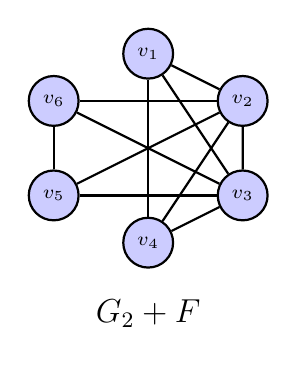
\begin{tikzpicture}
  [scale=.6, auto=left, 
   vertex/.style={circle, fill=blue!20, draw=black, thick, inner sep=2pt, minimum size=18pt},
   edge/.style={thick, draw=black},
   bold_edge/.style={line width=2.5pt, draw=black}]

  % Vértices
  \node[vertex] (n1) at (2,4) {$\scriptstyle v_1$};
  \node[vertex] (n2) at (4,3) {$\scriptstyle v_2$};
  \node[vertex] (n3) at (4,1) {$\scriptstyle v_3$};
  \node[vertex] (n4) at (2,0) {$\scriptstyle v_4$};
  \node[vertex] (n5) at (0,1) {$\scriptstyle v_5$};
  \node[vertex] (n6) at (0,3) {$\scriptstyle v_6$};

  % Aristas normales de G_2
  \foreach \from/\to in {n1/n2, n2/n3, n1/n3, n1/n4, n2/n4, n3/n4, n5/n6}
    \draw[edge] (\from) -- (\to);

  % Aristas reteñidas de F: {v3,v6}, {v3,v5}, {v2,v6}, {v2,v5}
  \foreach \from/\to in {n3/n6, n3/n5, n2/n6, n2/n5}
    \draw[edge] (\from) -- (\to);

  % Etiqueta inferior
    \node at (2,-1.5) {\large{$G_2 + F$}};
\end{tikzpicture}
